\documentclass[12pt]{article}
\usepackage[top=1in, bottom=1in, left=1in, right=1in]{geometry}

\usepackage{setspace}
\onehalfspacing

\usepackage{amssymb}
%% The amsthm package provides extended theorem environments
\usepackage{amsthm}
\usepackage{epsfig}
\usepackage{times}
\renewcommand{\ttdefault}{cmtt}
\usepackage{amsmath}
\usepackage{graphicx} % for graphics files
\usepackage{tabu}

% Draw figures yourself
\usepackage{tikz} 

% The float package HAS to load before hyperref
\usepackage{float} % for psuedocode formatting
\usepackage{xspace}

% from Denovo Methods Manual
\usepackage{mathrsfs}
\usepackage[mathcal]{euscript}
\usepackage{color}
\usepackage{array}

\usepackage[pdftex]{hyperref}
\usepackage[parfill]{parskip}

% math syntax
\newcommand{\nth}{n\ensuremath{^{\text{th}}} }
\newcommand{\ve}[1]{\ensuremath{\mathbf{#1}}}
\newcommand{\Macro}{\ensuremath{\Sigma}}
\newcommand{\rvec}{\ensuremath{\vec{r}}}
\newcommand{\vecr}{\ensuremath{\vec{r}}}
\newcommand{\omvec}{\ensuremath{\hat{\Omega}}}
\newcommand{\vOmega}{\ensuremath{\hat{\Omega}}}
\newcommand{\sigs}{\ensuremath{\Sigma_s(\rvec,E'\rightarrow E,\omvec'\rightarrow\omvec)}}
\newcommand{\el}{\ensuremath{\ell}}
\newcommand{\sigso}{\ensuremath{\Sigma_{s,0}}}
\newcommand{\sigsi}{\ensuremath{\Sigma_{s,1}}}
%---------------------------------------------------------------------------
%---------------------------------------------------------------------------
\begin{document}
\begin{center}
{\bf NE 155/255, Fall 2019\\
November 20, 2019 \\
Monte Carlo Variance Reduction
}
\end{center}

\textbf{Variance Reduction}\\
What we have talked about so far is \textit{analog} Monte Carlo:
\begin{itemize}
    \item Natural laws are \textbf{preserved}
    \item The game is the ``analog" of the physical problem of interest (the history of each particle is simulated exactly)
    \item No alteration of PDFs
    \item At collision, particle is killed if absorption
    \item Particle is born with weight 1
    \item weight unchanged throughout history
    \item Score when tallying events is 1
\end{itemize}
%
We often, instead, want to do \textit{non-analog} Monte Carlo:
\begin{itemize}
    \item To reduce computation time, the strict analog simulation of particles is abandoned
    \item Variance Reduction techniques: absorption suppression, roulette (history termination), splitting (history propagation), forced collisions, source biasing, hybrid methods
    \item Alter PDFs to favor events of interest
    \item Particle can have different birth weight
    \item Weight is altered if biased PDF is used
    \item Particle survives ``absorption" and weight is changed
    \item Splitting and RR can change weight
    \item Score current weight when tallying
\end{itemize}
%
We'll talk about implicit capture (AKA survival biasing), roulette, splitting, and weight window maps. 

The first thing to think about is how to measure success. How do we know if a calculation is ``better"?\\
We use the figure of merit
\[
FOM =\frac{1}{R^2 t}\:,
\]
where $R$ is the relative error and $t$ is the particle tracking time.\\
What we really want is to reduce both of these. \\
Why are they related to one another this way? Recall that $S_x \propto \sqrt{\frac{1}{N}}$.\\
It's clear that without variance reduction techniques to reduce error by a factor of two you need to increase particle count (and hence time) by a factor of four.\\
FOM measures if we're really winning.

\textit{The idea of VR is to track particles that will contribute meaningfully to the desired results and to avoid tracking those that will not while maintaining a fair game.}

\textbf{Categories of VR methods}\\
There are a huge number of VR methods out there. Some are simple, some are complicated. Some are easy to use, others are not. \\
\underline{Misuse of many of these methods can lead to incorrect answers without clear warning that the} \\\underline{answers are incorrect.}\\
Here is a list of common types of VR, but we'll go into detail of a very few. There are four main categories (using the MCNP manual as a reference here):
%
\begin{enumerate}
\item Truncation methods: cut off the parts of phase space you don't think you need
  \begin{itemize}
  \item geometry truncation
  \item energy cutoff
  \end{itemize}
  
\item Population Control methods: directly control the number and weight of particles
  \begin{itemize}
  \item splitting
  \item roulette
  \item executed a variety of ways: geometry-based splitting/roulette, energy-based splitting/roulette, weight windows, weight cutoff
  \end{itemize}

\item Modified Sampling methods: play games with the representation of physics to try to get better particle numbers and weights (alter underlying physical reality without biasing results)
  \begin{itemize}
  \item exponential transform
  \item survival biasing (implicit capture)
  \item forced collisions
  \item source biasing
  \item neutron-induced photon production biasing
  \end{itemize}

\item Partially Deterministic methods [Hazard!]: black magic; circumvent the normal random-walk process by using deterministic-like techniques. These methods can be combined to give results that look good and are completely wrong.
  \begin{itemize}
  \item point detectors
  \item DXTRAN
  \item correlated sampling
  \end{itemize}
\end{enumerate}

\textbf{Survival Biasing}\\
This is a very common technique. In analog MC, what happens when a particle undergoes a collision?
\[
\text{tally }w_i \qquad \text{and } w_{i+1} = 0
\]
If this particle's history is terminated, is it available to contribute to the answer and provide more data?\\
To keep it around, we'll just change the particle's weight in a way that preserves physics rather than terminate it. \\
What is the probability of an absorption during a collision in terms of macroscopic cross sections?
\[
P_{abs} = \frac{\Sigma_a}{\Sigma_t}
\]
We can use this to change particle weight and keep particles around for longer
\[
\text{tally }w_i*\frac{\Sigma_a}{\Sigma_t} \qquad \text{and } w_{i+1} = w_i*(1 - \frac{\Sigma_a}{\Sigma_t})
\]
The reduction in particle weight at each collision compensates, statistically, for the nonphysical scattering. This maintains a fair game and provides more information per history, though at the cost of each collision being worth less.

\textbf{Target Weight Map}\\
We can use the notion of weight to conduct VR. \\
What if we have a weight that is really \textit{low}? : wastes time\\
What if we have a weight that is really \textit{high}? : increases variance (relative error)\\
Ideally, we'd like to keep $w_{\min} \leq w \leq w_{\max}$.

When looking for a specific answer, some regions may be more important to the answer than others. We can make a map expressing the relative importances for a given problem (as we've alluded to). As particles move, they will traverse from regions of one importance to another. We can use how they change importance values to change their weight and the number of particles that we're tracking. We will talk about how you use these maps, and then about some ways to make them.

We can use the idea of importance to create the target weights where we'd like particles to exist and associated bounding values. We usually make a map of $w_{nom}$ and set $w_{\min}$ and $w_{\max}$ from there. 

%problem here - no definition of w_nom prior to its introduction in the above sentence

\textbf{Splitting}\\
If particles have too high a weight or are moving into a more important region we can split them into more particles with lower weights. We preserve the total weight to maintain a fair game:\\
\noindent\makebox[\linewidth]{\rule{\textwidth}{0.4pt}}
if $w_i > w_{\max}$:
\begin{itemize}
\item Split Ratio (SR) = $\frac{w_i}{w_{nom}}$
\item get $\xi$, a random number on [0, 1)
\item if $\xi \geq$ (SR - int(SR)):
  \begin{itemize}
  \item create int(SR) new particles
  \end{itemize}
\item else:
  \begin{itemize}
  \item create int(SR) + 1 new particles
  \end{itemize}
\item For all new particles, $w_{i+1} = \frac{w_i}{\# \text{new particles}}$
\end{itemize}
\noindent\makebox[\linewidth]{\rule{\textwidth}{0.4pt}}
%
You're preserving the total weight on average and converting 1 particle with too high a weight to multiple particles with a more useful weight and/or tracking more particles in an important part of the problem. 
%(draw picture of one large particle crossing into another region and becoming two or several smaller particles where size represents weight)

\clearpage

\textbf{Rouletting}\\
Conversely, if a particle has too low of a weight or is moving into a less important region, we can either increase its weight or kill it. Again, we preserve the total weight.\\
\noindent\makebox[\linewidth]{\rule{\textwidth}{0.4pt}}
if $w_i < w_{\min}$:
\begin{itemize}
\item Roulette Ratio (RR) = $\frac{w_i}{w_{nom}}$
\item get $\xi$, a random number on [0, 1)
\item if $\xi \geq$ RR:
  \begin{itemize}
  \item kill particle; $w_{i+1} = 0$
  \end{itemize}
\item else:
  \begin{itemize}
  \item $w_{i+1} = w_{nom}$
  \end{itemize}
\end{itemize}
\noindent\makebox[\linewidth]{\rule{\textwidth}{0.4pt}}
%
On average we're killing enough particles to make up for increasing the weight of some particles. We are taking low weight particles that we don't want to waste our time tracking and converting them to useful particles and/or tracking fewer particles in less important parts of the problem.
%(draw picture of several small particles crossing into another region and becoming one larger particle)

\begin{figure}[!htb]
\centering
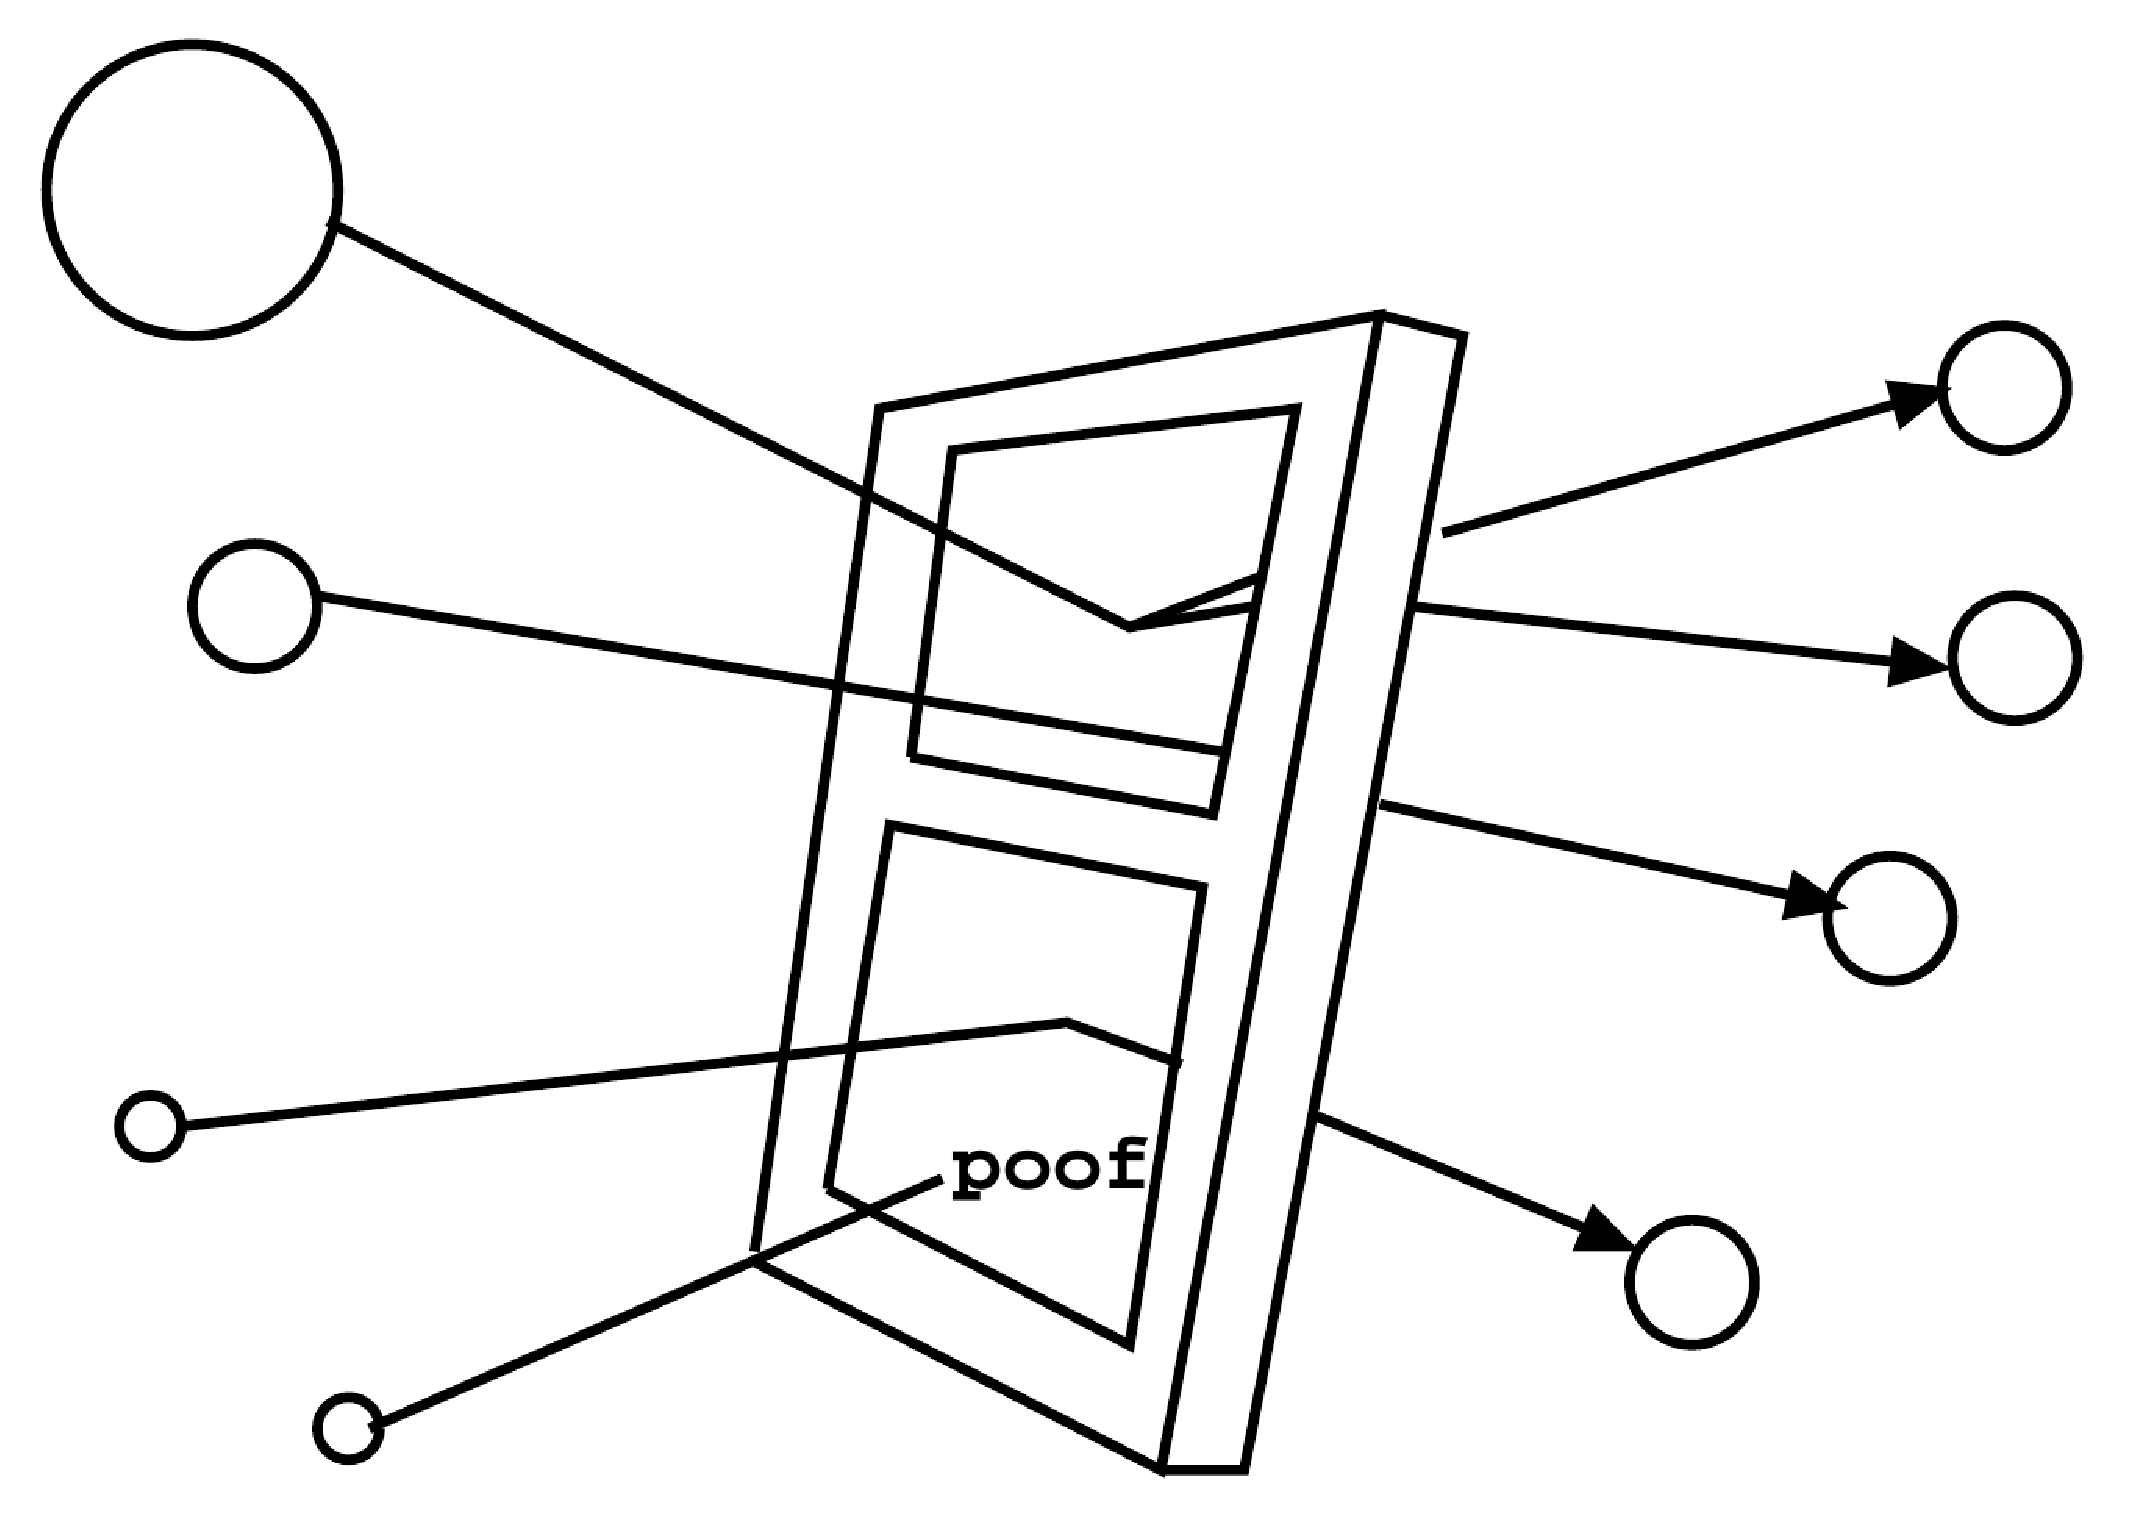
\includegraphics[width=0.7\textwidth]{fig/ww-mcnp.eps}
\caption{Weight window phase space splitting and roulette (from MCNP manual).}
\label{fig:ww}
\end{figure}

\end{document}